\documentclass{beamer}
\usepackage[utf8]{inputenc}
\usepackage[english]{babel}
\usepackage{helvet}
\usepackage[T1]{fontenc}
\usepackage{textcomp}
\usepackage[inline]{asymptote}
\usepackage{slide_helper}
\usepackage{multirow}
\usepackage{cellspace}
\usepackage{tikz}
\usepackage{subfigure}
\usetikzlibrary{shapes.geometric, arrows}
\usepackage{pgfplots}
\pgfplotsset{compat=1.5} 
\usepgfplotslibrary{statistics}
\usetikzlibrary{external}
\tikzexternalize%

\title[MA205 - Section 3.2]{Conditional Probability}

\DeclareSymbolFont{extraup}{U}{zavm}{m}{n}
\DeclareMathSymbol{\varheart}{\mathalpha}{extraup}{86}
\DeclareMathSymbol{\vardiamond}{\mathalpha}{extraup}{87}
\DeclareMathSymbol{\varclub}{\mathalpha}{extraup}{84} 
\DeclareMathSymbol{\varspade}{\mathalpha}{extraup}{85}

\newcommand{\suitheart}[1][]{{\color{red}\text{#1}\varheart}}
\newcommand{\suitspade}[1][]{{\color{black}\text{#1}\spadesuit}}
\newcommand{\suitdiamond}[1][]{{\color{red}\text{#1}\vardiamond}}
\newcommand{\suitclub}[1][]{{\color{black}\text{#1}\varclub}}
\newcommand{\card}[2]{{#1{\color{black}\text{#2}}}}

\newcommand{\prob}[1]{P\left(#1\right)}
\newcommand{\condprob}[2]{\prob{#1~\middle|~#2}}
\newcommand{\comb}[2]{_{#1}C_{#2}}

\newcommand\encircle[1]{%
  \tikz[baseline=(X.base)]  % chktex 36 chktex 1
    \node (X) [draw, shape=circle, inner sep=0, fill=yellow!10] {\strut #1};} % chktex 36 chktex 1

\begin{document}
\begin{frame}
\titlepage
\end{frame}

\begin{frame}
\begin{example}\label{ML classifier}
\vspace{-2mm}%beamer bug: extra space is added when a label is used, so this is to make this slide and the next look the same
The \dataset{photo\_classify} data set represents a machine learning algorithm classifying a sample of 1822 photos as either about fashion or not.\pause

\vspace{-1mm}
\begin{center}
\begin{tabular}{llccc}
&&\multicolumn{2}{c}{\variable{truth}} & \\\cline{3-4}
&&\outcome{fashion} & \outcome{not} & Total \\\cline{2-5}
\multirow{2}{*}{\variable{mach\_learn}} & \outcome{pred\_fashion} & 197 & 22 & 219 \\
&\outcome{pred\_not}& 112 & 1491 & 1603 \\\cline{2-5}
&Total & 309 & 1513 & 1822
\end{tabular}
\end{center}\pause

\question{If a photo is actually about fashion, what is the chance the algorithm will correctly identify the photo as being about fashion?}\pause
\answer{Of the 309 fashion photos, the algorithm correctly classifies 197 of them.

\vspace{-6mm}
\begin{equation*}
\prob{\small\text{\variable{mach\_learn} is \outcome{pred\_fashion} given \variable{truth} is \outcome{fashion}}}=\dfrac{197}{309} = 0.638
\end{equation*}}
\vspace{-3mm}
\end{example}
\end{frame}

\begin{frame}
\begin{example}
Using the same data set as in Example~\ref{ML classifier}.
\vspace{-2mm}
\begin{center}
\begin{tabular}{llccc}
&&\multicolumn{2}{c}{\variable{truth}} & \\\cline{3-4}
&&\outcome{fashion} & \outcome{not} & Total \\\cline{2-5}
\multirow{2}{*}{\variable{mach\_learn}} & \outcome{pred\_fashion} & 197 & 22 & 219 \\
&\outcome{pred\_not}& 112 & 1491 & 1603 \\\cline{2-5}
&Total & 309 & 1513 & 1822
\end{tabular}
\end{center}

\question{If the algorithm predicts the photo as being about fashion, what is the probability is actually is?}\pause
\answer{Of the 1603 photos predicted to be about fashion, 112 we actually about fashion.

\vspace{-8mm}
\begin{equation*}
\prob{\small\text{\variable{truth} is \outcome{fashion} given \variable{mach\_learn} is \outcome{pred\_fashion}}}=\dfrac{112}{1603} = 0.070
\end{equation*}}
\end{example}
\end{frame}

\begin{frame}
\begin{note}
It can be helpful to draw Venn Diagrams of these contingency tables using rectangles.
\end{note}\pause

\begin{example}
The Venn Diagram for Example~\ref{ML classifier} is:
\begin{center}
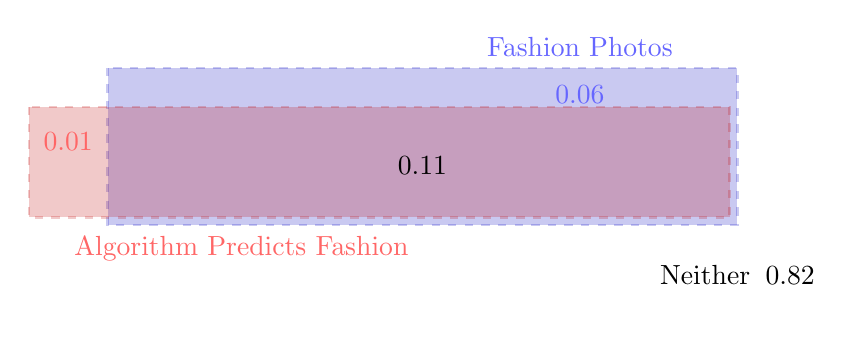
\begin{tikzpicture}
\draw[draw, dashed, fill=blue!40, blue!75!black, opacity=0.21, thick] (0,0) rectangle (8,-2);
\draw[draw, dashed, fill=red!40, red!75!black, opacity=0.21, thick] (-1,-0.5) rectangle (7.9,-1.9);
\node [label={[blue!60] Fashion Photos}] at (6,-0.1) {};
\node [label={[red!60] Algorithm Predicts Fashion}] at (1.7,-2.7) {};
\node [label={[red!60] 0.01}] at (-0.5,-1.3) {};
\node [label={[blue!60] 0.06}] at (6,-.7) {};
\node [label={[black] 0.11}] at (4,-1.6) {};
\node [label={[black] Neither\: 0.82}] at (8,-3) {};
\end{tikzpicture}
\end{center}
\end{example}
\end{frame}

\begin{frame}
\begin{definition}
A \textbf{marginal probability} is a probability based on a single variable without regard to other variables.
\end{definition}\pause

\begin{example}
\begin{equation*}
\prob{\small\text{\variable{mach\_learn} is \outcome{pred\_fashion}}} = \dfrac{219}{1822} = 0.12
\end{equation*}\pause
\vspace{-3.5mm}
\end{example}

\begin{definition}
A probability of outcomes for two or more variables is called a\\ \textbf{joint probability}.
\end{definition}\pause

\begin{example}
\vspace{-4mm}
\begin{equation*}
\prob{\small\text{\variable{mach\_learn} is \outcome{pred\_fashion} and \variable{truth} is \outcome{fashion}}} = \dfrac{197}{1822} = 0.11
\end{equation*}
\vspace{-4.5mm}
\end{example}
\end{frame}

\begin{frame}
\begin{note}
Sometimes a comma is substituted for \textquote{and} in a joint probability.

\vspace{-1mm}
\begin{center}
\begin{tabular}{c}
$\prob{\small\text{\variable{mach\_learn} is \outcome{pred\_fashion}, \variable{truth} is \outcome{fashion}}}$ \\
means the same thing as \\
$\prob{\small\text{\variable{mach\_learn} is \outcome{pred\_fashion} and \variable{truth} is \outcome{fashion}}}$
\end{tabular}
\end{center}
\end{note}
\end{frame}

\begin{frame}
\begin{definition}
A \textbf{table proportions} is a table that summarizes joint probabilities. The proportions are computed by dividing each count by table's total.
\end{definition}\pause

\begin{example}\label{table props}
\vspace{-2mm}%beamer bug: extra space is added when a label is used, so this is to make this slide and the next look the same
The table proportions for \dataset{photo\_classify} are:

\vspace{-5mm}
\begin{center}
%\addtolength{\cellspacetoplimit}{1.5pt}
%\addtolength{\cellspacebottomlimit}{1.5pt}
\begin{tabular}{Sl Sr Sr Sr}\hline
& \variable{truth}: \outcome{fashion} & \variable{truth}: \outcome{not} & Total \\\hline
\variable{mach\_learn}: \outcome{pred\_fashion} & $\tfrac{197}{1822}$  & \visible<3->{$\tfrac{22}{1822}$} & \visible<4->{$\tfrac{219}{1822}$} \\[1mm]
\variable{mach\_learn}: \outcome{pred\_not} & \visible<5->{$\tfrac{112}{1822}$} & \visible<6->{$\tfrac{1491}{1822}$} & \visible<7->{$\tfrac{1603}{1822}$} \\\hline
Total & \visible<8->{$\tfrac{309}{1822}$} & \visible<9->{$\tfrac{1513}{1822}$} & \visible<10->{$\tfrac{1822}{1822}$} \\\hline
\multicolumn{4}{c}{$\downarrow~\downarrow~\downarrow$}\\\hline
& \variable{truth}: \outcome{fashion} & \variable{truth}: \outcome{not} & Total \\\hline
\variable{mach\_learn}: \outcome{pred\_fashion} & 0.1081  & \visible<3->{0.0121} & \visible<4->{0.1202} \\
\variable{mach\_learn}: \outcome{pred\_not} & \visible<5->{0.0615} & \visible<6->{0.8183} & \visible<7->{0.8798} \\\hline
Total & \visible<8->{0.1696} & \visible<9->{0.8304} & \visible<10->{1.0} \\\hline
\end{tabular}
\end{center}
\end{example}
\end{frame}

\begin{frame}
\begin{example}
The table proportions from Example~\ref{table props} make a probability distribution.
\begin{center}
\begin{tabular}{lc}\hline
Joint Outcome & Probability \\\hline
\variable{mach\_learn} is \outcome{pred\_fashion} and  \variable{truth} is \outcome{fashion} & 0.1081 \\
\variable{mach\_learn} is \outcome{pred\_fashion} and  \variable{truth} is \outcome{not} & 0.0121\\
\variable{mach\_learn} is \outcome{pred\_not} and  \variable{truth} is \outcome{fashion} & 0.0615\\
\variable{mach\_learn} is \outcome{pred\_not} and  \variable{truth} is \outcome{not} & 0.8182\\\hline
\end{tabular}
\end{center}
\end{example}\pause

\begin{note}
Joint probabilities can be used to calculate marginal probabilities in simple cases.
\end{note}\pause

\begin{example}\small
\vspace{-4mm}
\begin{equation*}
\begin{aligned}
\prob{\small\text{\variable{truth} is \outcome{fashion}}}
&= \prob{\small\text{\variable{mac\_learn} is \outcome{pred\_fashion} and \variable{truth} is \outcome{fashion}}} \\
&\qquad +\prob{\small\text{\variable{mac\_learn} is \outcome{pred\_not} and \variable{truth} is \outcome{fashion}}} \\\pause
&=0.1081 + 0.0615 \pause
= 0.1696
\end{aligned}
\end{equation*}
\end{example}
\end{frame}
\end{document}
